
Our objective is to explore the impact of shipping costs fluctuations on different firm variables. Using the sample built by \textcite{barrot_globalization_2019} and Compustat firm level information. We estimate the following specification at the firm-year level for the 133 different industries:  

\[Y_{ijt} = \beta_{j0} + \beta_{j1}\Delta SC_{it} + \beta_{j2}\Delta GDP_{it} +\alpha_{i} + \delta_{t} +u_{ijt} \quad for\quad j\in \{2000,\dots,3999\}\]

\begin{equation}
 Y_{i,j,t} = \beta_{0} + \beta_{1}\Delta SC_{j,t} +u_{i,j,t}   
\end{equation}

\begin{equation}
 Y_{i,j,t} = \beta_{0} + \beta_{1}\Delta SC_{j,t}+\beta_{2}\Delta GDP_{t}+\alpha_{i}+u_{i,j,t}   
\end{equation}

where $Y_{ijt}$ is the changes of sales to total assets, the inventory to total assets, the gross profit margin or the net profit margin, depending on which firm level variable we want to test. On the right hand side, we have our variable of interest the $\Delta SC$ estimating the sensitivity of the firm variables to it. Also, we added the GDP growth to proxy the business cycle and firm and time fixed effects to control for unobserved characteristics.  

The following four plots show the values of the relevant beta against the average SC for each industry. We can see that there is not any major trend throughout the different shipping costs levels. From the lower to the upper part the beta fluctuates around zero, 
with its sign constantly changing. This can lead us to concluded that our variable of interest captures a different behaviour than the one used by \textcite{barrot_globalization_2019}.

\begin{figure}[htbp]
	\centering
		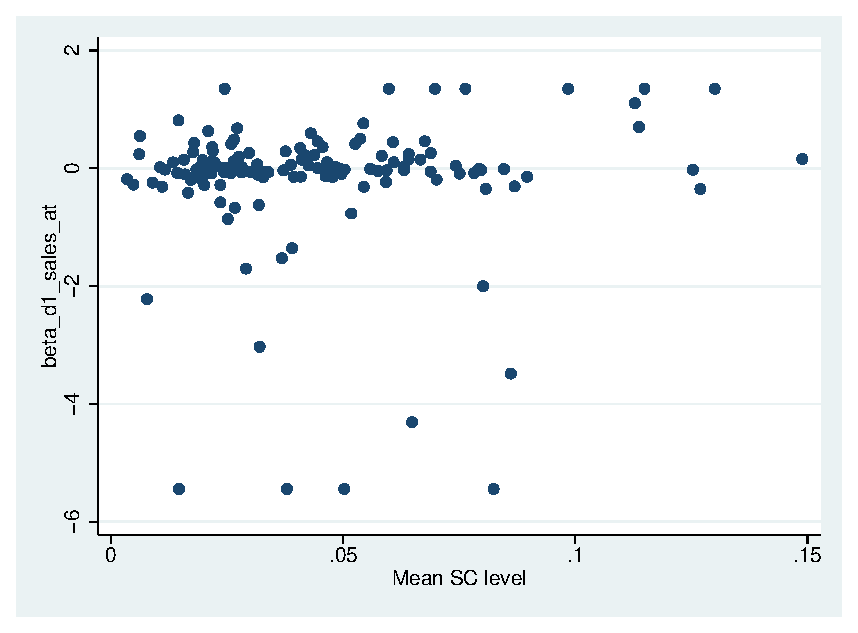
\includegraphics[width=4.5in]{beta_sales.eps}
	\caption{SC relation with $\beta^{\Delta SC}_{t}$ for $\Delta$ Sales/Total assets by industry.}
	\label{panel_sales}
\end{figure}


\begin{figure}[htbp]
	\centering
		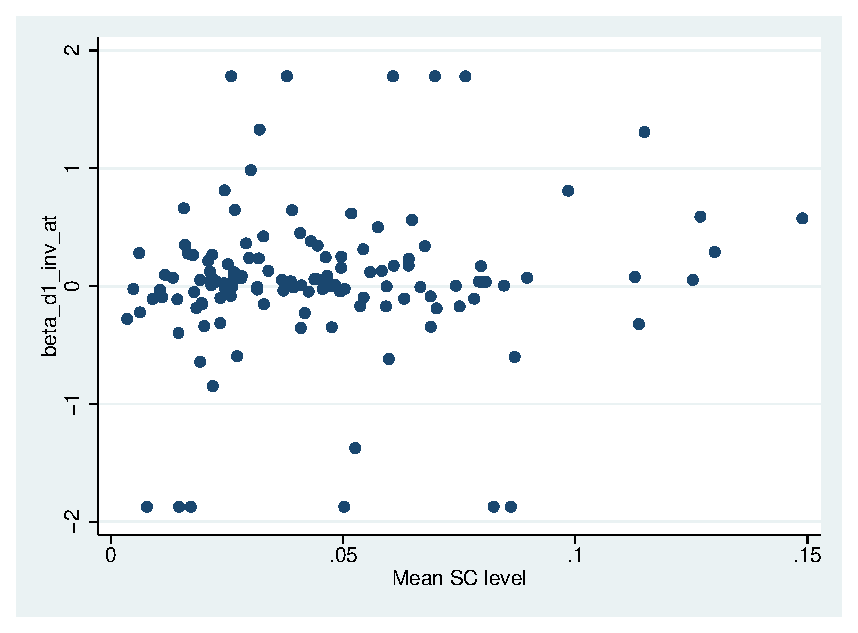
\includegraphics[width=4.5in]{beta_inv.eps}
	\caption{SC relation with $\beta^{\Delta SC}_{t}$ for $\Delta$ inventory/total assets by industry.}
	\label{panel_inv}
\end{figure}


\begin{figure}[htbp]
	\centering
		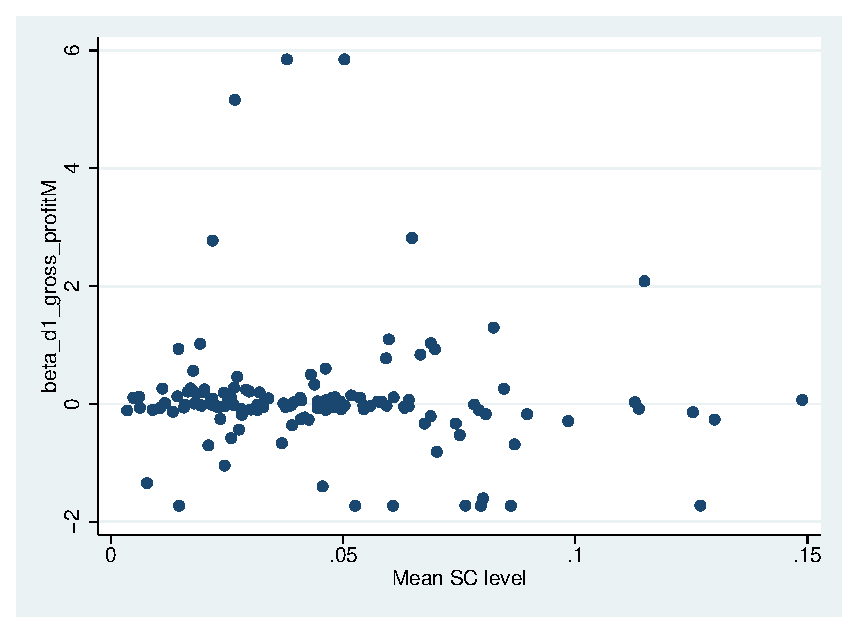
\includegraphics[width=4.5in]{beta_gross_profit.eps}
	\caption{SC relation with $\beta^{\Delta SC}_{t}$ for $\Delta$ gross Profit Margin by industry.}
	\label{panel_gross}
\end{figure}

\newpage
\begin{figure}[htbp]
	\centering
		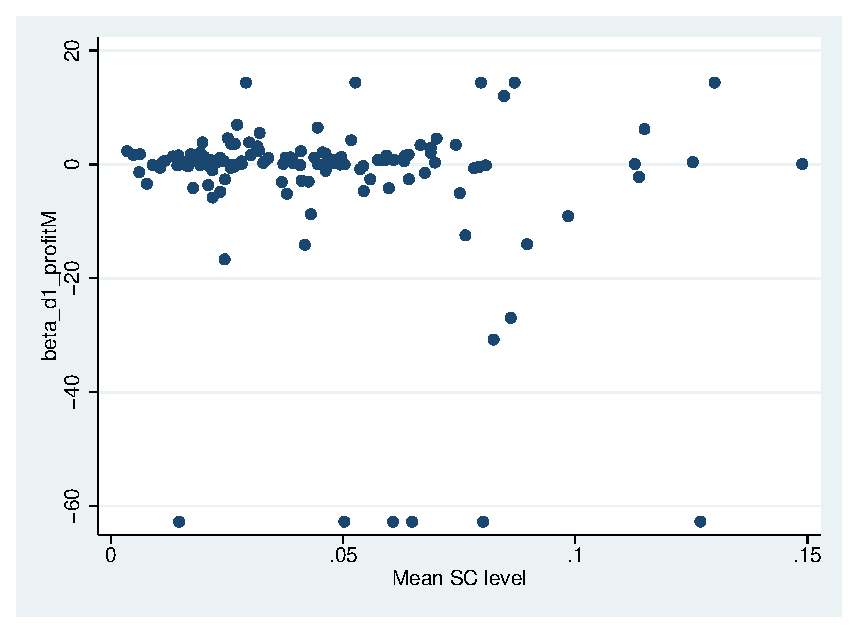
\includegraphics[width=4.5in]{beta_profit.eps}
	\caption{SC relation with $\beta^{\Delta SC}_{t}$ for $\Delta$ Net Profit Margin by industry.}
	\label{panel_profit}
\end{figure}

The tables \ref{table:tables} and \ref{table:tables2} reported the coefficients from that regressions that are significant and its respective industry and average SC. Again, we verify the beta's changing sign for the bottom and top part of the SC distribution. Reinforcing the idea that this variable catches a different behaviour. 
\renewcommand{\arraystretch}{1.2}
\begin{table}[htbp!]\centering
\def\sym#1{\ifmmode^{#1}\else\(^{#1}\)\fi}

\caption{Panel regression with $\Delta SC$ for the equation above.}
\label{table:tables}
\begin{tabular}{l*{1}{cccccc}}
\hline\hline
                    &\multicolumn{4}{c}{}                                                         \\
                    &       SIC &        Mean SC&          $\beta^{\Delta SC}_{st}$&        \textit{t-statistic}\\
\hline
\textbf{$\Delta$ Inventory/Total Assets}&&&&&&\\

&2821 &	.0475067&	-.3494209&	-3.345888\\
&3823 &	.0200592&	-.3399673&	-2.410894\\
&3842 &	.0194549&	-.142437&	-2.399844\\
&...&...&...&...\\
&3452&	.0675484&	.3390469&	2.171849\\
&3241&	.1488986&	.5757623&	2.473763\\
&3677&	.0300618&	.9844124&	2.609636\\
&3728&	.0115665&	.0957699&	2.633406\\
&3567&	.0407185&	.450414&	2.669905\\
&3826&	.0158724&	.3498243&	2.918991\\
&2273&	.0543087&	.3131082&	3.520694\\
&2052&	.0697474&	1.781317&	8.772565\\

\hline
\textbf{$\Delta$ Sales/Total Assets}&&&&&&\\
&2085&	.0389743&	-1.356233&	-21.3461\\
&3851&	.0318048&	-.6211227&	-3.24739\\
&3713&	.0319606&	-3.03007&	-3.097911\\
&3674&	.0088988&	-.2413746&	-2.981573\\
&2835&	.0165453&	-.4128631&	-2.936528\\
&3842&	.0194549&	-.1847367&	-2.53145\\
&2111&	.0290345&	-1.702453&	-2.463537\\
&3221&	.0801065&	-2.002049&	-2.238723\\
&3724&	.0047644&	-.2758157&	-2.143154\\
&...&...&...&...\\
&3672&	.0297061&	.2614544&	2.165365\\
&3861&	.021774&	.3611721&	2.186076\\
&2024&	.1300146&	1.350973&	2.386137\\
&2844&	.0375627&	.2885819&	2.880985\\
&3579&	.0264701&	.4897395&	3.249883\\
&2033&	.1128187&	1.106375&	3.834811\\
&2273&	.0543087&	.7648988&	6.788162\\


\hline\hline
\end{tabular}
\end{table}
\renewcommand{\arraystretch}{1.2}
\begin{table}[htbp!]\centering
\def\sym#1{\ifmmode^{#1}\else\(^{#1}\)\fi}

\caption{Panel regression with $\Delta SC$ for the equation above.}
\label{table:tables2}
\begin{tabular}{l*{1}{cccccc}}
\hline\hline
                    &\multicolumn{4}{c}{}                                                         \\
                    &       SIC &        Mean SC&          $\beta^{\Delta SC}_{st}$&        \textit{t-statistic}\\
\hline
\textbf{$\Delta$ Gross Profit Margin}&&&&&&\\
&3452&	.0675484&	-.3335997&	-2.846541\\
&2086&	.1253107&	-.1417454&	-2.708851\\
&...&...&...&...\\
&3524&	.0461743&	.6002178&	2.094328\\
&3442&	.0608425&	.1130603&	2.124526\\
&3571&	.0144866&	.9349212&	2.473737\\
&3579&	.0264701&	.2760885&	2.615221\\
&3613&	.0218559&	2.772453&	3.853394\\
&3944&	.0666275&	.8373231&	3.918834\\

\hline
\textbf{$\Delta$ Net Profit Margin}&&&&&&\\
&2531&	.0896&	-14.02558&	-8.019841\\
&3652&	.0416979&	-14.11668&	-2.96984\\
&3221&	.0801065&	-62.76466&	-2.846039\\
&2673&	.0648116&	-62.76466&	-2.42098\\
&3562&	.0245114&	-2.629872&	-2.073061\\
&2511&	.0984547&	-9.111079&	-2.002404\\
&...&...&...&...\\
&3843&	.0196577&	3.876543&	2.661499\\
&3334&	.0846151&	12.00757&	3.91942\\
&2024&	.1300146&	14.38218&	4.022253\\
\hline\hline
\end{tabular}
\end{table}
